%
% 04_einfache_polygone.tex -- Einfuhrung in den Satz von Jordan fuer einfache Polygone
%
% (c) 2026 Dominik Castelberg, Ostschweizer Fachhochschule
%
% !TEX root = ../../buch.tex
% !TEX encoding = UTF-8
%

\section{Der Fall einfacher Polygone
\label{jordan:section:einfache_polygone}}
\kopfrechts{Der Fall einfacher Polygone}

Einfache Polygone verwerfen die Einschränkng der Konvexität und erlauben es, dass die Kurve in sich selbst zurückkehrt, solange sie sich nicht schneidet. 
Die Eigenschaft der Konvexität war jedoch in der vorherigen Beweisführung entscheidend, da sie die Definition der konvexen Hülle und die Trennung der Ebene in zwei Gebiete erleichtert hat. 

Wir benötigen daher einen neuen Ansatz, um die bisherigen, durch die Eigenschaften der Konstruktion der behandelten Körper gegebenen, Definitionen für ``Innen'' und ``Aussen'' neu zu formulieren.
Wertvolle Werkzeuge sind hierbei die Strahlenparität und die dazugehörige Paritätsinvarianz.

\begin{definition}[Strahlenparität\label{jordan:definition:strahlenparitaet}]
    Sei $P$ ein einfaches Polygon und $p \in \mathbb{R}^2 \setminus \partial P$ ein Punkt, der nicht auf $\partial P$ liegt.
    Für jeden Strahl $L$ mit Anfangspunkt $p$, der keine Ecke von $P$ trifft und nicht entlang einer Kante von $P$ verläuft, sei $N(p,L)$ die Anzahl Schnittpunkte von $L$ mit $\partial P$ 
    und $N(p,L) \mod 2$
die \emph{Strahlenparität}
\index{Strahlenparitat@Strahlenparität}%
oder
die \emph{Parität} dieser Anzahl.
\end{definition}


\begin{lemma}[Paritätsinvarianz\label{jordan:lemma:paritaetsinvarianz}]
    Sei $\gamma_{pq}$ eine Kurve, die zwei verschiedene Punkte $p$ und $q$ in der Ebene $\mathbb{R}^2$ verbindet und $\gamma_{pq} \cap \partial P = \emptyset$.  
    Dann haben $p$ und $q$ die gleiche Strahlenparität.
\end{lemma}

\begin{figure}
    \centering
    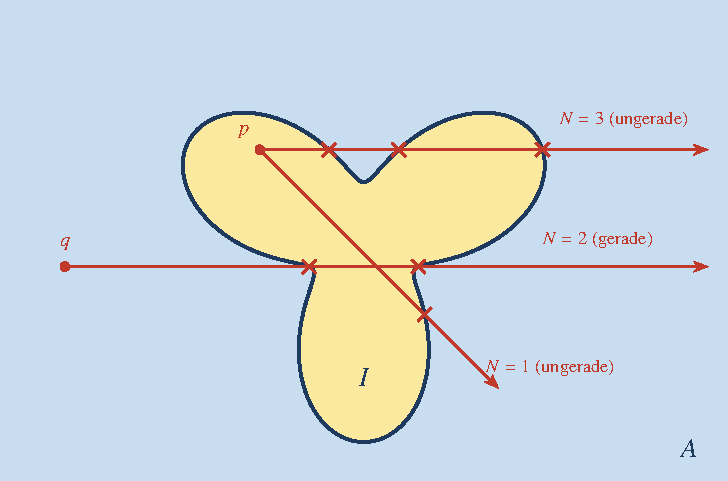
\includegraphics{papers/jordan/images/strahlenparitaet.pdf}
    \caption{Strahlenparität am Beispiel einer Jordan-Kurve.}
\end{figure}

Das Konzept der Strahlenparität und deren Invarianz erlaubt es uns, die Punkte in der Ebene in zwei Mengen zu unterteilen: diejenigen, die eine gerade Anzahl von Schnittpunkten mit dem Polygon haben (die äussere Menge), und diejenigen, die eine ungerade Anzahl von Schnittpunkten haben (die innere Menge).

\begin{definition}[Innen- und Aussengebiet\label{jordan:definition:innen_und_aussengebiet}]
    Sei $P$ ein einfaches Polygon und $p \in \mathbb{R}^2 \setminus \partial P$. 
    Dann gilt:
    \begin{itemize}
        \item $p$ liegt im inneren Gebiet $I$ von $P$, wenn $N(p,L)$ ungerade ist.
        \item $p$ liegt im äusseren Gebiet $A$ von $P$, wenn $N(p,L)$ gerade ist.
    \end{itemize}
\end{definition}

Damit der Satz von Jordan für einfache Polygone gilt, müssen noch weitere Eigenschaften von $I$ und $A$ aufgezeigt werden.

\begin{itemize}
    \item $I$ und $A$ sind beide offen und nicht leer.
    \item $I$ und $A$ sind wegzusammenhängend.
    \item $I$ ist beschränkt, während $A$ unbeschränkt ist.
    \item $P$ ist der gemeinsame Rand von $I$ und $A$.
\end{itemize}


\subsubsection{Offenheit von $I$ und $A$
\label{jordan:subsubsection:offenheit_innen_aussen}}

\begin{lemma}[Offenheit von $I$ und $A$\label{jordan:lemma:offenheit_innen_aussen}]
    Wenn $P$ ein einfaches Polygon ist, dann sind $I$ und $A$ offen.
\end{lemma}

Der Beweis für die Offenheit von $I$ und $A$ basiert auf der lokalen Konstanz der Strahlenparität.
Die Parität $N(p, L) \mod 2$ ist lokal konstant in $p$ für sämtliche gültigen Strahlen $L$, sofern $p$ nicht auf dem Polygon liegt.
Wir können daher immer einen Punkt $p' \in I$ oder $p' \in A$ in der Nähe von $p$ finden, sodass $N(p', L) \mod 2 = N(p, L) \mod 2$ für alle gültigen Strahlen $L$ gilt.

\subsubsection{Wegzusammenhang von $I$ und $A$
\label{jordan:subsubsection:wegzusammenhang_innen_aussen}}

\begin{lemma}[Wegzusammenhang von $I$ und $A$\label{jordan:lemma:wegzusammenhang}]   
        Sei $P$ ein einfaches Polygon, $I$ das innere Gebiet von $P$ und $A$ das äussere Gebiet von $P$. 
        Dann sind $I$ und $A$ wegzusammenhängend.
\end{lemma}

Die Etablierung des Wegzusammenhangs von $I$ und $A$ verlangt ein topologisch substantielleres Argument: Die Wegzusammenhangseigenschaften von triangulierten Polygonen. 

\begin{definition}[Triangulierung eines einfachen Polygons\label{jordan:definition:triangulierung_einfaches_polygon}]
    Eine \emph{Triangulierung} eines einfachen Polygons $P$ ist eine Zerlegung von $P$ in nicht überlappende Dreiecke, deren Ecken jeweils Ecken von $P$ sind und die sich paarweise nur in Kanten oder Ecken schneiden.
\index{Triangulierung}%
\end{definition}


\begin{satz}[Triangulierungssatz für einfache Polygone\label{jordan:satz:triangulierung_einfaches_polygon}]
    Jedes einfache Polygon $P$ mit $n \geq 3$ Ecken besitzt eine Triangulierung.
\end{satz}

Dieser Triangulierungssatz wurde 1975 von G. H. Meisters\cite{jordan:meisters1975} präzise bewiesen.
Der Beweis basiert auf folgendem Lemma:

\begin{lemma}[Existenz einer Diagonale\label{jordan:lemma:existenz_diagonale}]
    Jedes einfache Polygon $P$ mit $n \geq 4$ Ecken besitzt eine Diagonale, d.h. eine Linie, die zwei nicht benachbarte Ecken von $P$ verbindet und vollständig innerhalb von $P$ liegt.
\end{lemma}

Die Existenz einer in einem Polygon mit mehr als drei Ecken liegenden Diagonale impliziert, dass das Polygon in zwei kleinere Polygone zerlegt werden kann.


\begin{figure}
    \centering
    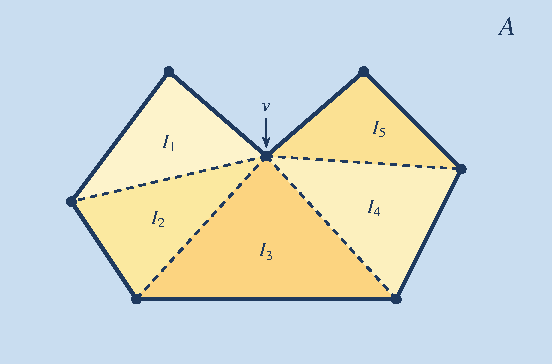
\includegraphics{papers/jordan/images/triangulierung.pdf}
    \caption{Triangulierung eines einfachen Polygons in nicht überlappende Dreiecke an Reflexpunkt $v$.}
\end{figure}

Mit dieser Triangulierung können wir nun den Wegzusammenhang zwischen zwei Punkten in $I$ aufzeigen.
Da $I$ als Vereinigung von anliegenden Dreiecken dargestellt werden kann, und Dreiecke als konvexe Polygone inherent wegzusammenhängend sind, können wir einen Weg zwischen zwei Punkten in $I$ konstruieren, indem wir die Dreiecke durchqueren, die das Polygon bilden.

\subsubsection{Beschränktheit von $I$
\label{jordan:subsubsection:beschraenktheit_innen}}

\begin{lemma}[Beschränktheit von $I$ \label{jordan:lemma:beschraenktheit_innen}]
    Sei $P$ ein einfaches Polygon und $I$ das innere Gebiet von $P$. 
    Dann ist $I$ beschränkt.
\end{lemma}

Der Beweis der Beschränktheit von $I$ ist relativ trivial und basiert darauf, dass eine konvexe Hülle mit endlichen Ecken beschränkt ist und man für jedes einfache Polygon eine konvexe Hülle finden kann.
Das Innere eines konvexen Polygons ist beschränkt, da das Polygon aus einer endlichen Anzahl von Ecken besteht und entsprechend immer von einem Kreis mit genug grossem Radius vollständig umschlossen werden kann.
Da dieser selbst Kreis beschränkt ist, ist auch das Innere des Polygons, als Teilmenge des Kreises, ebenfalls beschränkt.

Die endliche Anzahl von Ecken garantiert auch, dass die konvexe Hülle eines einfachen Polygons konstruiert werden kann.

\subsubsection{Unbeschränktheit von $A$
\label{jordan:subsubsection:unbeschraenktheit_aussen}}

\begin{lemma}[Unbeschränktheit von $A$ \label{jordan:lemma:unbeschraenktheit_aussen}]
    Sei $P$ ein einfaches Polygon und $A$ das äussere Gebiet von $P$. 
    Dann ist $A$ unbeschränkt.
\end{lemma}

Die Unbeschränktheit von $A$ ist elementar.
Da $\mathbb{R}^2 = I \cup P \cup A$ und sowohl $I$ als auch $P$ beschränkt sind, muss $A$ unbeschränkt sein, damit $\mathbb{R}^2$ unbeschränkt ist.

\subsubsection{Nicht-Leerheit von $I$
\label{jordan:subsubsection:nicht_leerheit_innen}}

\begin{lemma}[Nicht-Leerheit von $I$\label{jordan:lemma:nicht_leerheit_innen}]
        Sei $P$ ein einfaches Polygon und $I$ das innere Gebiet von $P$. 
        Dann ist $I$ nicht leer.
\end{lemma}

Die nicht-Leerheit von $I$ kann aus einem geometrischen Argument abgeleitet werden: Jedes Polygon mit $n \geq 3$ Ecken muss eine nicht-leeres, inneres Gebiet haben.
Wie schon in \ref{jordan:subsubsection:wegzusammenhang_innen_aussen} gezeigt, kann jedes Polygon mit $n \geq 3$ Ecken in nicht überlappende Dreiecke zerlegt werden.
Da jedes Dreieck ein nicht-leeres inneres Gebiet hat, kann das innere Gebiet des Polygons nicht leer sein, da es die Vereinigung der inneren Gebiete der Dreiecke ist.

\subsubsection{Nicht-Leerheit von $A$
\label{jordan:subsubsection:nicht_leerheit_aussen}}

\begin{lemma}[Nicht-Leerheit von $A$\label{jordan:lemma:nicht_leerheit_aussen}]
    Wenn $P$ ein einfaches Polygon ist, dann ist $A$ nicht leer.
\end{lemma}

Die nicht-Leerheit von $A$ kann aus der Unbeschränktheit von $A$ abgeleitet werden, da eine leere Menge beschränkt ist.

\subsubsection{$P$ als gemeinsamer Rand von $I$ und $A$
\label{jordan:subsubsection:gemeinsamer_rand_innen_aussen}}

\begin{lemma}[$P$ als gemeinsamer Rand von $I$ und $A$\label{jordan:lemma:gemeinsamer_rand}]   
        Sei $P$ ein einfaches Polygon, $I$ das innere Gebiet von $P$ und $A$ das äussere Gebiet von $P$. 
        Dann ist $P$ der gemeinsame Rand von $I$ und $A$.
\end{lemma}

Der Beweis dafür, dass $P$ der gemeinsame Rand von $I$ und $A$ ist, wird in zwei Schritten durchgeführt.
Erst wird gezeigt, dass jeder Punkt auf $P$ ein Randpunkt von $I$ und $A$ ist, und dann wird gezeigt, dass kein Punkt auf dem Rand von $I$ und $A$ nicht auf $P$ liegt.

Für den ersten Schritt können wir eine Eigenschaft sämtlicher $p \in P$ verwenden: Um jeden dieser Punkte können wir einen beliebig kleinen Kreis zeichnen.
Da $p$ auf einer Kante liegt, teilt diese Kante den Kreis lokal in zwei Hälften.
Wenn wir nun je einen Strahl von einem beliebigen Punkt innerhalb beider Hälften in eine beliebige gültige Richtung ziehen, werden sie unterschiedliche Paritäten haben und somit auf unterschiedlichen Seiten des Randes sein.
Daher muss sich $p$ auf dem Rand von $I$ und $A$ befinden.

Für den zweiten Schritt nutzen wir eine Eigenschaft aller Punkte $x$, die nicht auf $P$ liegen.
Da $P$ eine geschlossene Menge endlich vieler Segmente ist, gibt es einen minimalen positiven Abstand $d$ zwischen $x$ und $P$.
Wir können einen Kreis um $x$ mit Radius $0 < r < d$ zeichnen, der $P$ nicht schneidet.
Alle Punkte innerhalb dieses Kreises haben entsprechend die gleiche Parität gegenüber $P$.
Das heisst, dass sämtliche Punkte innerhalb dieses Kreises entweder alle in $I$ oder alle in $A$ liegen.
Daher kann $x$ nicht auf dem Rand von $I$ und $A$ liegen.


\subsection{Der Satz von Jordan für einfache Polygone
\label{jordan:subsection:satz_von_jordan_einfache_polygone}}

Hiermit haben wir gezeigt, dass sämtliche Voraussetzungen für die Gültigkeit des Satzes von Jordan für den Fall einfacher Polygone erfüllt sind.
Mit der Strahlenparität haben wir ein effizientes Werkzeug gefunden, welches für polygonale Jordan-Kurven beliebig einsetzbar ist.